\section{Estado del arte}
%Estado del arte: El estado del arte de un objeto de estudio se refiere al estado más elevado de desarrollo alcanzado por el objeto en un momento particular. En este caso el objeto de estudio es la solución del problema, que puede ser un producto de software, un método, un modelo, una teoría, etc. Se presenta el ámbito o la(s) principal(es) disciplina(s) que aborda(n) soluciones al problema (redes neuronales, informática médica, seguridad en redes, sistemas cooperativos, industria informática, etc.). Se espera una revisión de los fundamentos teóricos del objeto de estudio, los antecedentes que hay del tema expresado en dos formas, primero una breve descripción de su evolución y luego una descripción resumida del estado del arte actual (últimos años), desde dos perspectivas: nacional e internacional. Lo más importante es el estado del arte al día de hoy.

En esta sección se busca presentar los antecedentes y el estado actual sobre los dispositivos de retroalimentación vibrotáctil disponibles en el mercado, las cuales suelen venir con herramientas para el desarrollo de aplicaciones de terceros. Una de las herramientas que se le suelen facilitar a los desarrolladores es el SDK (\textit{Software Development Kit}), el cual es un conjunto de herramientas utilizadas para desarrollar aplicaciones proporcionadas por proveedores de hardware y software. Los SDK suelen estar compuestos por interfaces de programación de aplicaciones APIs (\textit{Application Program Interface}), código de muestra, documentación, entre otros elementos \citep{techopedia-SDK}. En la Tabla \ref{table:SDKs} muestra una comparativa de distintas características de los SDKs del mercado referente a dispositivos de \textit{haptic feedback}. Es importante señalar que el SDK no posee soporte multiplataforma, tampoco tiene una integración directa con Unity, sería necesario hacer un plugin para ello.

% ... /table-generation/sdk-comparation.tgn
\begin{table}[H]
\centering
\caption[Comparación SDK de distintos Guantes]{Comparación SDK de distintos Guantes \\Fuente: Elaboración propia (2018)}
\label{table:SDKs}
\begin{tabular}{|l|l|l|l|l|}
\hline
          & \begin{tabular}[c]{@{}l@{}}Lenguajes \\ soportados\end{tabular} & SO soportado                                                                  & \begin{tabular}[c]{@{}l@{}}Información \\ Bidireccional\end{tabular} & \begin{tabular}[c]{@{}l@{}}Integración \\ SDK con Unity\end{tabular} \\ \hline
OpenGlove & C\#, Java, JavaScript                                           & Windows                                                                       & SI                                                                   & \begin{tabular}[c]{@{}l@{}}NO\\ (Requiere plugin)\end{tabular}       \\ \hline
GloveOne  & C++ y C\#                                                       & \begin{tabular}[c]{@{}l@{}}Windows, MAC, \\ Linux, Android e iOS\end{tabular} & SI                                                                   & SI                                                                   \\ \hline
AvatarVR  & C++ y C\#                                                       & \begin{tabular}[c]{@{}l@{}}Windows, MAC,\\ Linux, Android e iOS\end{tabular}  & SI                                                                   & SI                                                                   \\ \hline
Dexmo     & No anunciado                                                    & No anunciado                                                                  & SI                                                                   & Si                                                                   \\ \hline
\end{tabular}
\end{table}


\subsection{OpenGlove}
	Es un proyecto que consiste en un dispositivo que entrega \textit{haptics feedback}. Fue pensado para dispositivos de realidad virtual e interfaces naturales. El proyecto partió en el 2014 con el propósito  de facilitar la construcción y flexibilizar uno de los recursos claves para la inmersión en ambientes de  realidad virtual \citep{openglove-info-page}. OpenGlove se ha pensado para que pueda ser utilizado en conjunto con otros dispositivos, como Oculus Rift, Kinect y Leap Motion. Por otra parte, los prototipos de OpenGlove, utilizan motores configurables con diferentes niveles de potencia, lo que permite la respuesta vibrotáctil en distintas áreas de la mano. Esto puede ser utilizado para representar la sensación de tocar objetos en entornos virtuales, como también, recibir retroalimentación que represente impacto, el cual sería útil en un juego de boxeo por ejemplo.   Actualmente, se soporta el uso de actuadores, sensores de flexibilidad y Unidad de Medición Inercial (IMU por sus siglas en inglés).
    
            
\begin{figure}[H]
  \begin{center} 
   	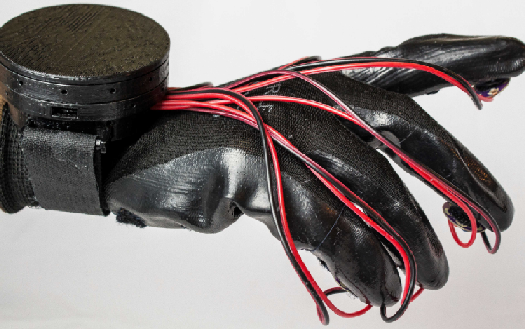
\includegraphics[width=0.5\textwidth]{images/fig-analisis-solucion/openglove.png} 
    \caption[Guantes OpenGlove]{Guantes OpenGlove \\Fuente: \cite{openglove-info-page}} 
    \label{fig:OpenGlove}
  \end{center}
\end{figure}

%\subsection{GloveOne}
% Now neurodigital only sell AvatarVR versión
%	Es un guante diseñado por Neurodigital para ofrecer la sensación del contacto con objetos en entornos de realidad virtual mediante  \textit{haptic feedback}. Posee 10 actuadores  vibrotáctiles distribuidos en posiciones fijas en los dedos, posee cinco sensores flexibles para el seguimiento de los dedos, se conecta mediante Bluetooth 4.0, posee una batería de litio con una duración de 8 horas. El guante posee un costo que van desde los 299 \euro \space . Las licencias profesionales alcanzan precios desde los  3.300 \euro \space hasta 13.300 \euro  \space la versión premium,  permiten acceder a la documentación, SDK y soporte, entre otros servicios.  \footnote{Precio de GloveOne y licencias: \url{https://www.neurodigital.es/gloveone/}}
    

%\begin{figure}[H]
%  \begin{center} 
%   	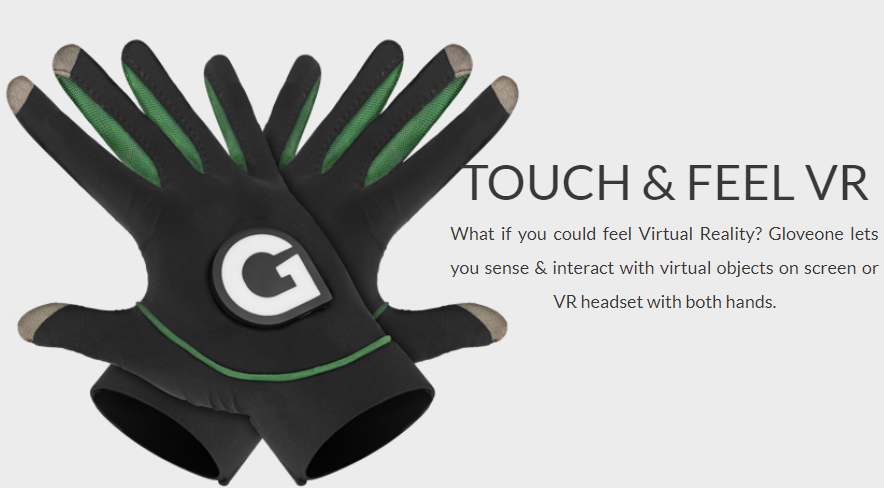
\includegraphics[width=0.4\textwidth]{images/fig-analisis-solucion/globeone.png} 
 %   \caption[Guantes GloveOne]{Guantes GloveOne \\Fuente: \cite{gloveone-info-page}} 
 %  \label{fig:gloveone}
 % \end{center}
%\end{figure}

    
\subsection{AvatarVR}
    	AvatarVR es otro guante diseñado por Neurodigital e incluye todas las funcionalidades presentes en GloveOne, junto a unas capacidades adicionales que ofrecen más funcionalidades. Además de los guantes se incluye un accesorio llamado TrackBand, que permite la captura de movimiento de la parte superior del cuerpo, basada en una configuración minimalista de los sensores  para en brazos y manos. Además sensores para el seguimiento de dedos mediante sensores 6x 9-AXIS IMUs. El guante y las trackbands poseen un costo desde 1.100 \euro \space.  Las licencias son de dos tipos profesional a 3.300 \euro \space y premium  a 13.300 \euro  \space para acceder a la documentación, SDK, soporte, entre otros servicios. 
	\footnote{Precio AvatarVR y licencias: \url{https://www.neurodigital.es/avatarvr/}}
        
\begin{figure}[H]
  \begin{center} 
   	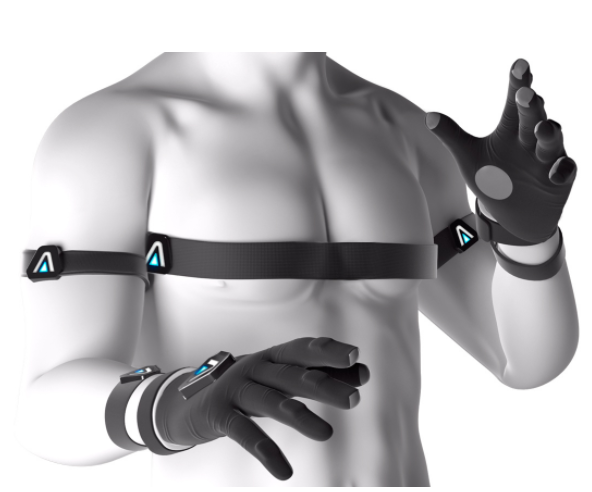
\includegraphics[width=0.4\textwidth]{images/fig-analisis-solucion/avatar-VR.png} 
     \caption[Guantes AvatarVR y TrackBand]{Guantes AvatarVR y TrackBand \\Fuente: \cite{avatarvr-info-page}} 
    \label{fig:avatarVR}
  \end{center}
\end{figure}

        
\subsection{Dexmo} 
    Dexmo es un exoesqueleto que permite \textit{haptic feedback} en ambientes de realidad virtual. Esto lo logra mediante la capacidad de retroalimentación de fuerza, lo que permite al usuario sentir el tamaño y la forma de cualquier objeto digital, lo que mejora enormemente la inmersión. La rigidez variable se logra mediante un control preciso del motor. Con esta característica, cada objeto virtual puede tener su propia rigidez.
    
Por protección de propiedad intelectual, su SDK sólo es accesible a clientes que hayan comprado Dexmo DK1. %En la figura se aprecian las capturas de lo que contiene sería una vista previa de su SDK.
    
            
\begin{figure}[H]
  \begin{center} 
   	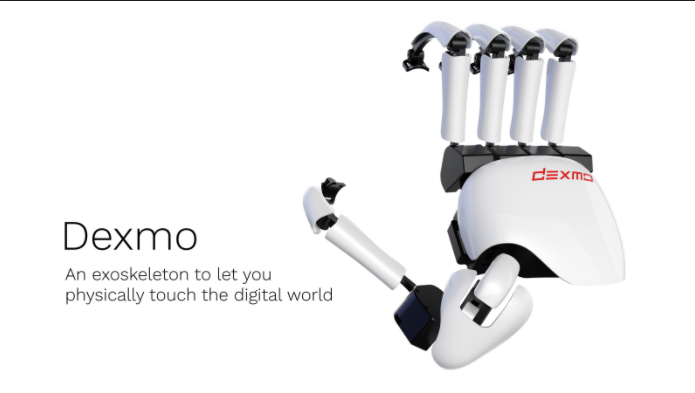
\includegraphics[width=0.5\textwidth]{images/fig-analisis-solucion/dexmo.png} 
    \caption[Guantes Dexmo]{Guantes Dexmo \\Fuente: \cite{dexmo-info-page}}  
    \label{fig:dexmo}
  \end{center}
\end{figure}
    
\subsection{Manus VR}
	Manus VR es un guante que permite \textit{haptic feedback}, seguimiento de dedos y manos para ambientes de realidad virtual. Sus especificaciones comerciales establecen que, es lavable, permite el seguimiento de los brazos, que también incluye un IMU para medir la orientación de la mano. Manus VR puede ser adquirido en dos versiones, la de desarrollador con un precio de 1.990 \euro \space y una versión profesional con un precio de 4.990 \euro \space \footnote{Precio de Manus VR y licencias \url{https://manus-vr.com/order.php}}
    
\begin{figure}[H]
  \begin{center} 
   	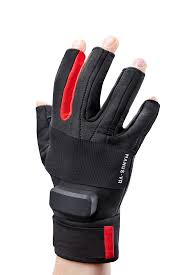
\includegraphics[width=0.3\textwidth]{images/fig-analisis-solucion/manus-vr.jpeg} 
    \caption[Guantes Manus VR]{Guantes Manus VR \\Fuente: \cite{manusvr-info-page}} 
    \label{fig:manus-vr}
  \end{center}
\end{figure}

\subsection{Haptx}
%Este es nuevo, muy interesante ...
%“HaptX Gloves are the result of years of research and development in haptic technology,” said Jake Rubin, Founder and CEO, HaptX Inc. “What really sets HaptX Gloves apart is the unprecedented realism they deliver. Our patented microfluidic technology physically displaces the skin the same way a real object would when touched, closely replicating its texture, shape, and movement.” 
\footnote{ Haptx \url{https://haptx.com/}}

\subsection{Sense glove}
\footnote{Sense Glove: \url{https://www.senseglove.com/}}

\subsection{Virtual Reality Smart Glove}
\footnote{VR Smart Glove: \url{http://www.designpartners.com/projects/virtual-reality-smart-glove/
}}

